\chapter{Вычислительные эксперименты. Проверка работоспособности модели}\label{ch:ch4}

В первую очередь необходимо проверить адекватность вышеизложенного подхода на модельных данных во всех режимах работы автомагистрали.
В данном разделе проводится два типа экспериментов~--- на модельных и на реальных данных, оба призваны проверить поведение модели в различных конфигурациях дорожной сети.

Эксперименты на модельных данных сводятся к проверке поведение модели на соответствие реально наблюдаемым процессам на простейших сегментах транспортной сети~--- прямой дороге, стыке двух дорог, съезд с автомагистрали, въезд на автомагистраль.
Графики представляют из себя тепловые карты по оси $x$ которой отложено расстояние от начала участка магистрали, по оси $y$~-- время.
В конце автомагистрали всегда находится небольшая ветвь представляющий из себя сток.

Эксперименты на реальных данных проводятся для участка МКАД между 99 и 101 километром с помощью расположенных на этом участке автомагистрали дорожных датчиков.
Один из датчиков используется для генерации автомобилей на въезде в моделируемый участок магистрали, второй~--- для верификации результатов.
Проводятся два эксперимента~--- эксперимент с моделированием прямой дороги и эксперимент с виртуальным перекрытием одной из полос магистрали.
В первом эксперименте рассчитывается показатель среднеквадратической ошибки
\[
    S = \sqrt{\frac{1}{K}\sum_{k=1}^K (n(k) - \bar{n}(k)},
\]
где $K$~--- число временных интервалов, $\bar{n}$~--- зафиксированное дорожным датчиком число проехавших по участку магистрали АТС с целью верификации результатов моделирования на реальных данных.

\section{Модельные данные}
\subsection{Прямая дорога}
Для начала рассмотрим поведение модели для простой пятиполосной дороги длиной 6 километров без перекрестков с линейно нарастающим вплоть до 150 АТС/мин потоком изображенное на фиг.~\ref{fig:simple_road}. В модели данная дорога представлена тремя ветвями по 2 километра.
Данный эксперимент показывает, что в модели нет существенных краевых эффектов на стыке ветвей.
\begin{figure}[ht]
    \begin{subfigure}[b][][b]{1.0\textwidth}
       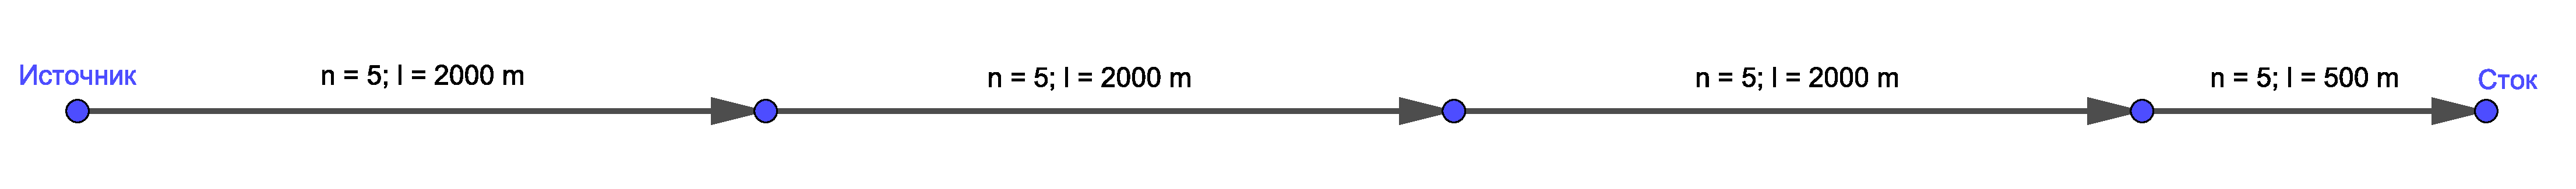
\includegraphics[width=1.0\linewidth]{scheme_simple_3block_road.eps}
       \caption{}
    \end{subfigure}

    \begin{subfigure}[b][][b]{1.0\textwidth}
       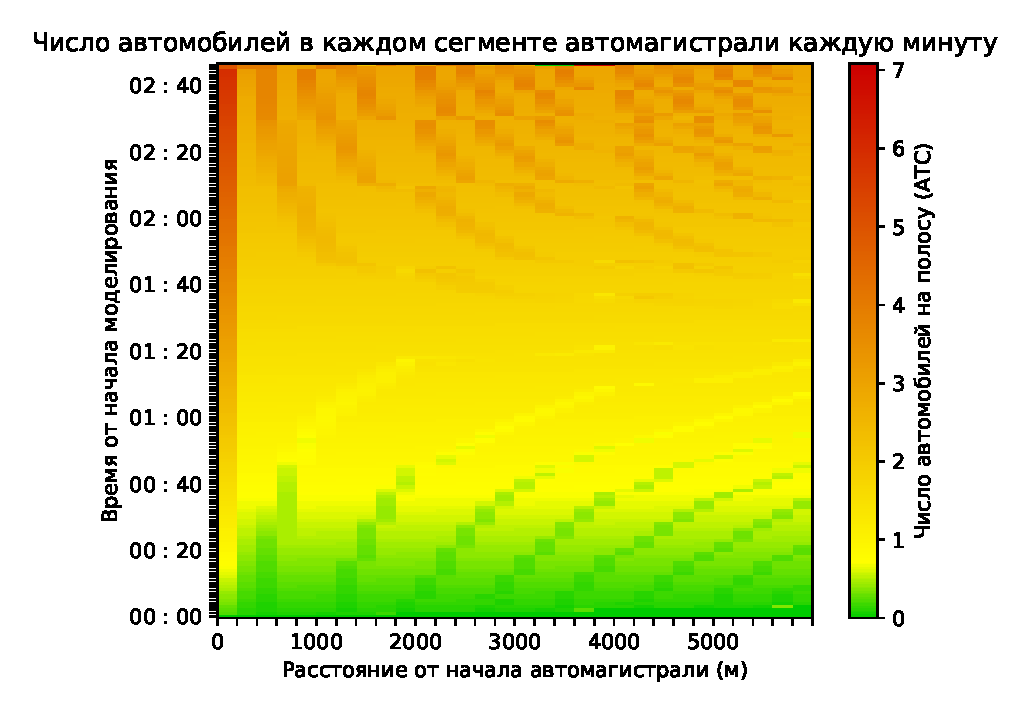
\includegraphics[width=1.0\linewidth]{simple_3_block_road.eps}
       \caption{}
    \end{subfigure}

    \caption{а) Схема простой дороги в модели состоит из 3 сегментов по 2 километра. б) Тепловая карта автомобилей на простой дороге без перекрестков с линейно нарастающим вплоть до 150 АТС/мин потоком.}
    \label{fig:simple_road}
\end{figure}

\subsection{Прямая дорога с сужением и синусоидальным потоком}
Для следующего эксперимента возьмем прямой участок пятиполосной дороги с сужением до двухполосной.
В данном эксперименте с целью рассмотрения как процесса формирования затора, так и его исчезновения пустим на вход синусоидальный поток с периодом равным времени моделирования и амплитудой в 85 АТС/мин.
Результат моделирования можно наблюдать на фиг.~\ref{fig:jammed_5-2_3block_road_sin_wave}.
На графике видно, что при уменьшении потока на сегменте, соответствующем двухполосной дороге, наблюдается разрыв потока АТС, который мы связываем с групповыми эффектами модели.
\begin{figure}[ht]
    \begin{subfigure}[b][][b]{1.0\textwidth}
       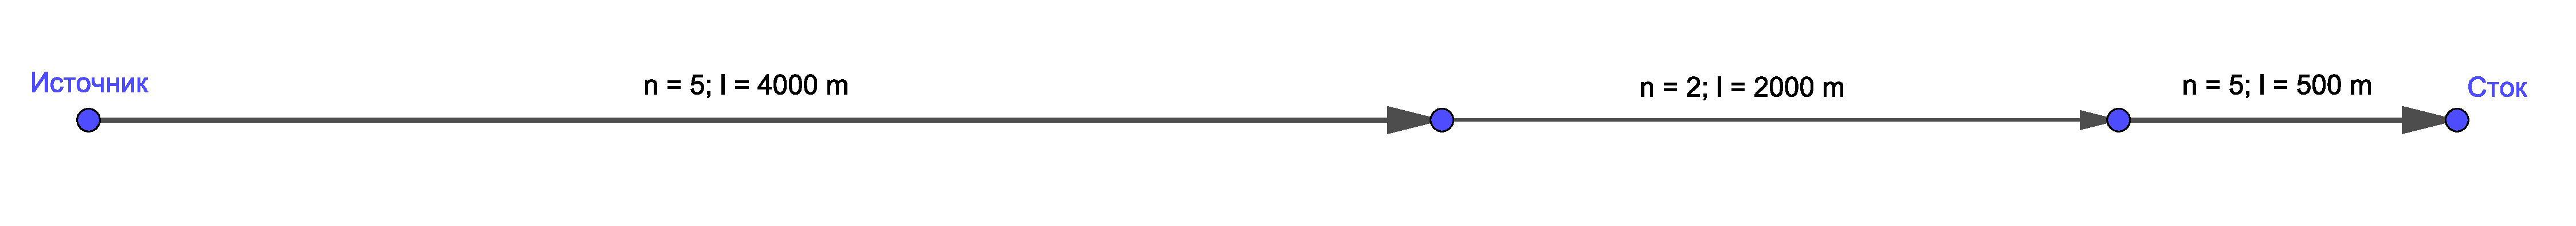
\includegraphics[width=1.0\linewidth]{scheme_jammed_sin_wave.eps}
       \caption{}
    \end{subfigure}

    \begin{subfigure}[b][][b]{1.0\textwidth}
       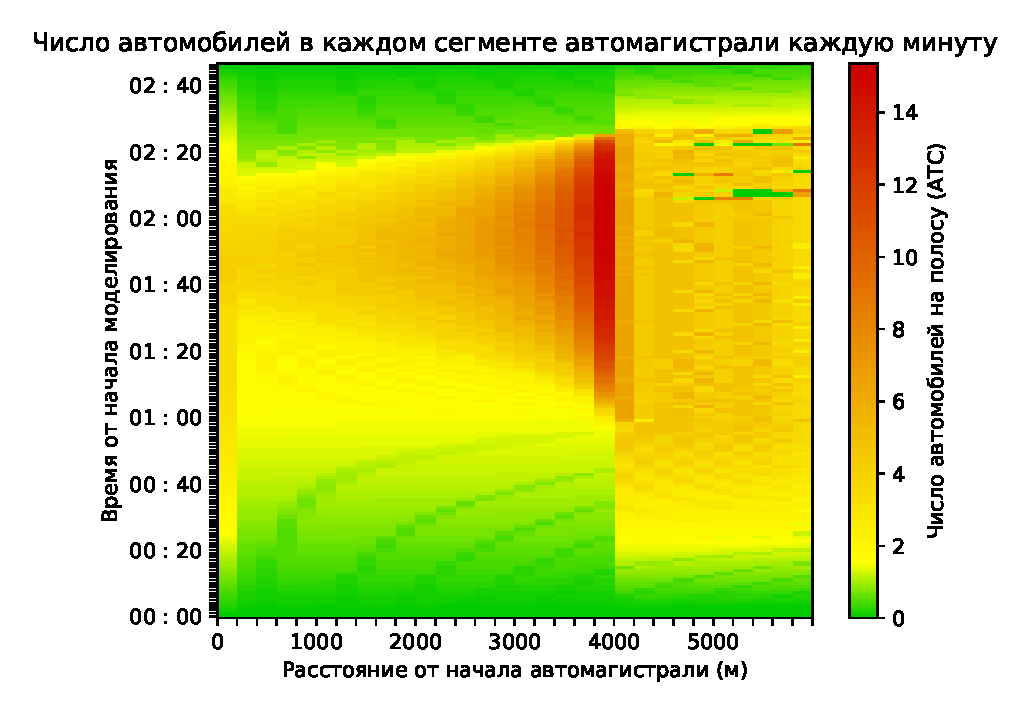
\includegraphics[width=1.0\linewidth]{jammed_5-2_3block_road_sin_wave.eps}
       \caption{}
    \end{subfigure}

    \caption{а) Схема дороги. б) Тепловая карта автомобилей на пятиполосной дороге без перекрестков с сужением до двух полос и синусоидальным потоком на входе.}
    \label{fig:jammed_5-2_3block_road_sin_wave}
\end{figure}

\subsection{Прямая дорога с пропадающим сужением}
Также рассмотрим ситуацию, когда при постоянном потоке в 100 АТС/мин на пятиполосной дороге с сужением до двухполосной данное сужение в середине моделирования пропадает.
Такая ситуация может сложиться, например, при прекращении ремонтных работ или устранении аварии. Результаты моделирования можно наблюдать на фиг.~\ref{fig:jammed_5-2_3block_road_with_unjam}.
\begin{figure}[ht]
    \begin{subfigure}[b]{1.0\textwidth}
       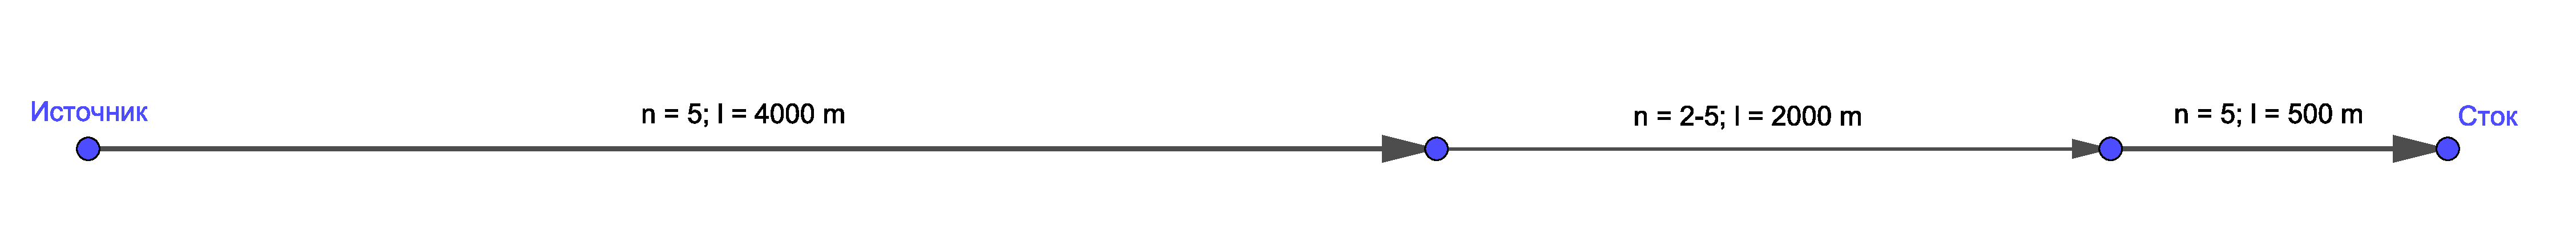
\includegraphics[width=1.0\linewidth]{scheme_jammed_with_unjam.eps}
       \caption{}
    \end{subfigure}

    \begin{subfigure}[b]{1.0\textwidth}
       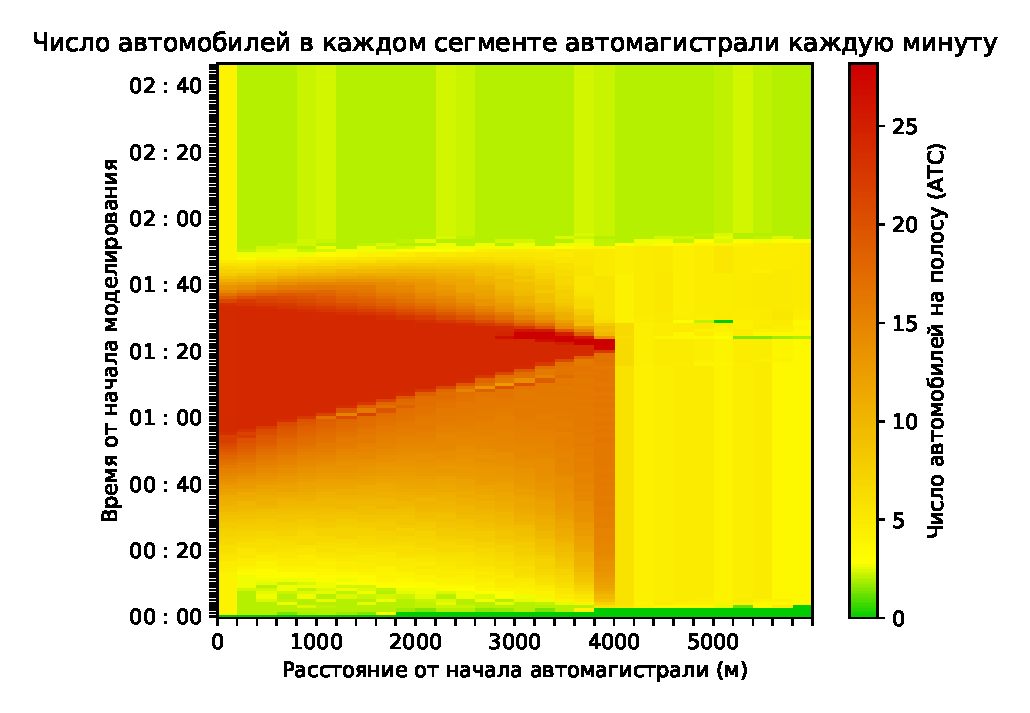
\includegraphics[width=1.0\linewidth]{jammed_5-2_3block_road_with_unjam.eps}
       \caption{}
    \end{subfigure}

    \caption{а) Схема дороги. б) Тепловая карта автомобилей на пятиполосной дороге без перекрестков с сужением до двух полос пропадающим в середине моделирования и постоянным потоком в 100 АТС/мин.}
    \label{fig:jammed_5-2_3block_road_with_unjam}
\end{figure}

\subsection{Перекресток со съездом}
Промоделируем оба варианта перекрестков возможных в предложенной модели.
Перекресток со съездом и перекресток с въездом. В обоих случаях основная автомагистраль -- пятиполосная. Въезд или съезд однополосные.

В эксперименте со съездом входной поток -- 65 АТС/мин. Доля съезжающих автомобилей линейно растет с 20\% до 60\%. На фиг.~\ref{fig:jamming_crossroad_exit_5_1} видно, что из за недостаточной пропускной способности съезда на основной автомагистрали образуется пробка.
\begin{figure}[ht]
    \begin{subfigure}[b]{1.0\textwidth}
       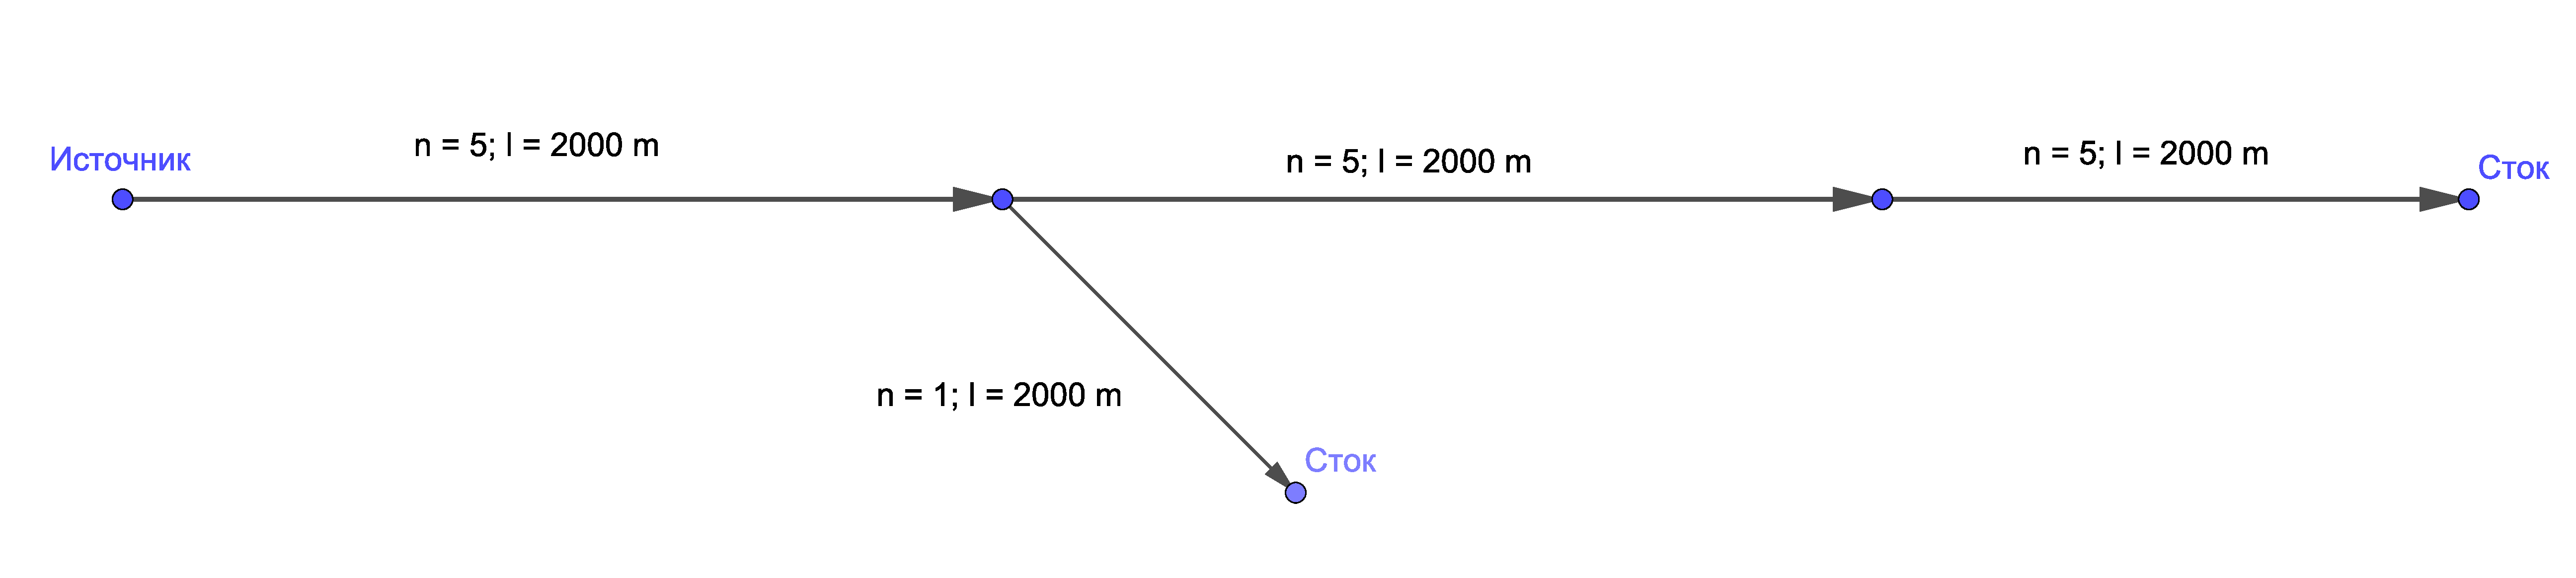
\includegraphics[width=1.0\linewidth]{scheme_jammed_crossroad_exit.eps}
       \caption{}
    \end{subfigure}

    \begin{subfigure}[b]{1.0\textwidth}
       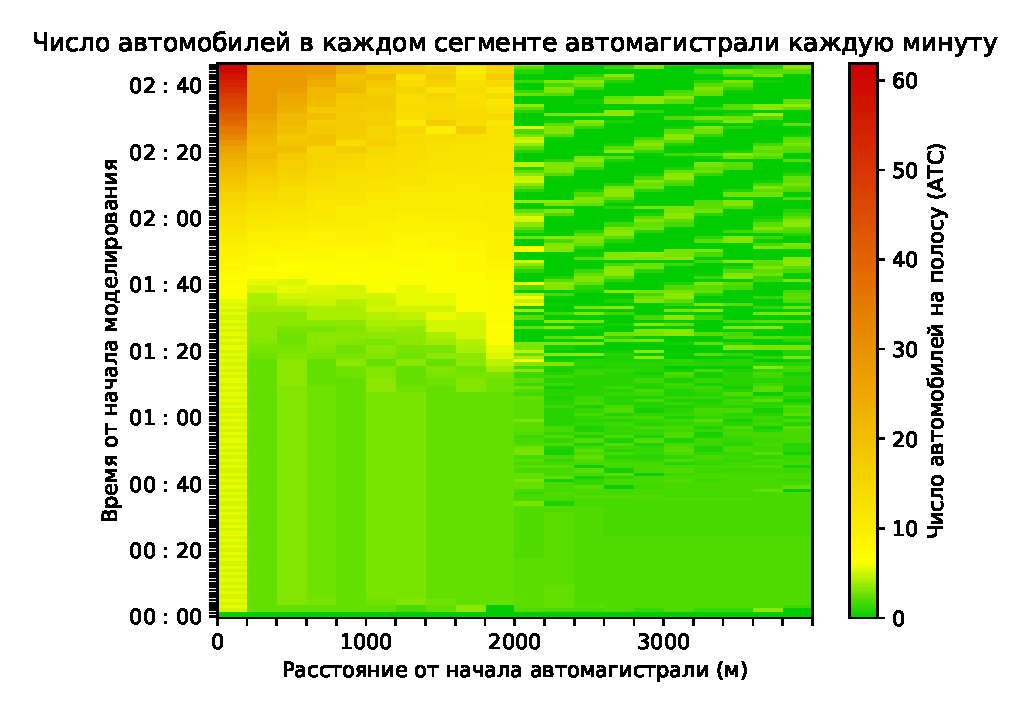
\includegraphics[width=1.0\linewidth]{jamming_crossroad_exit_5_1.eps}
       \caption{}
    \end{subfigure}

    \caption{а) Схема дороги. б) Тепловая карта автомобилей на пятиполосной дороге со съездом.}
    \label{fig:jamming_crossroad_exit_5_1}
\end{figure}

\subsection{Перекресток с въездом}
В эксперименте со въездом поток на автомагистрали~--- 140 АТС/мин, поток на въезде линейно растет от 20 до 50 АТС/мин. В данном случае также образуется пробка на основной автомагистрали, что видно на фиг.~\ref{fig:jamming_crossroad_enter_5_1}.
\begin{figure}[ht]
    \begin{subfigure}[b]{1.0\textwidth}
       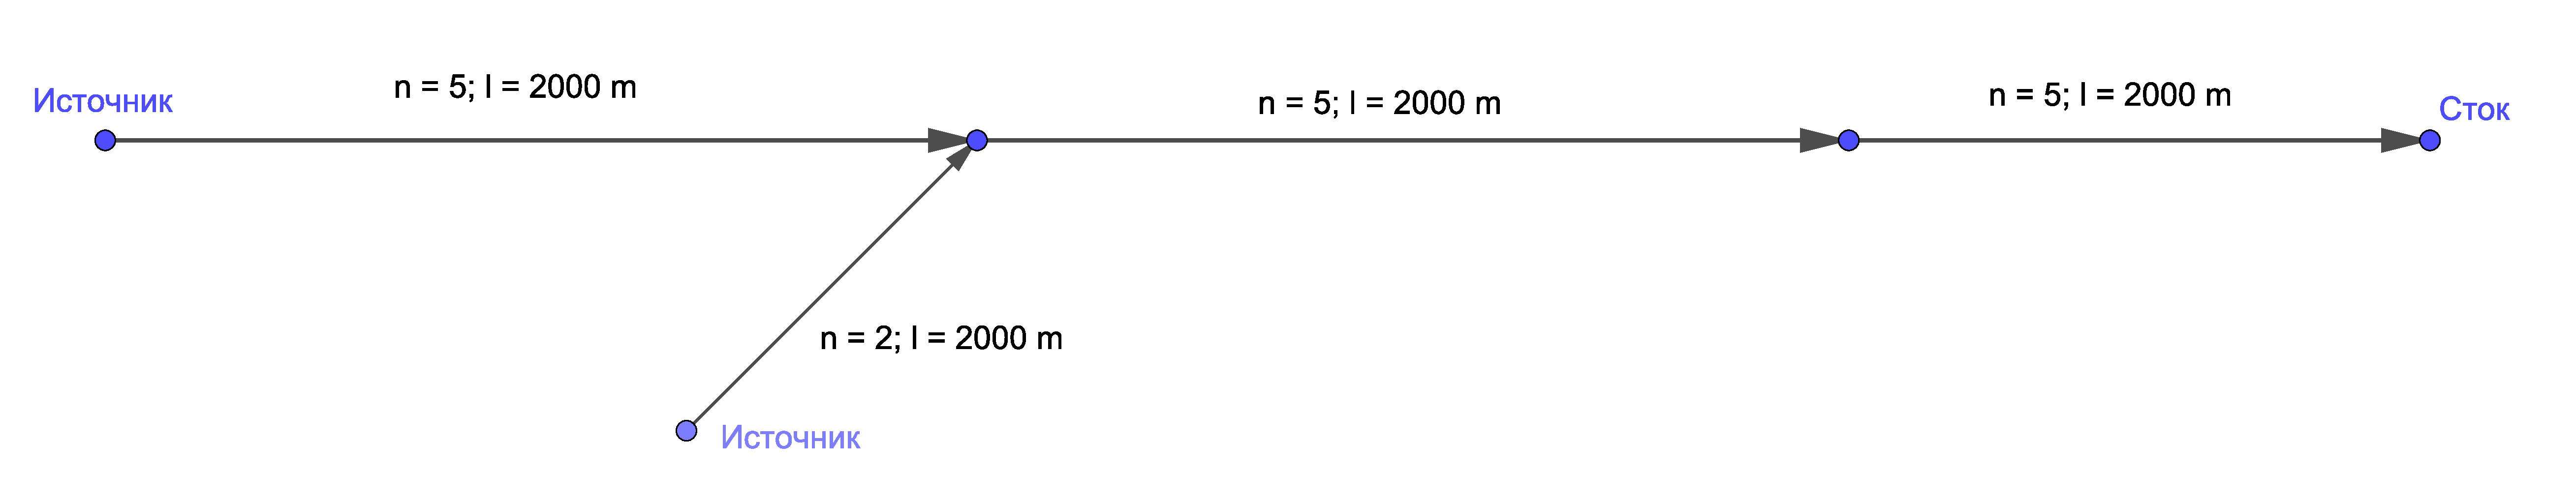
\includegraphics[width=1.0\linewidth]{scheme_jammed_crossroad_enter.eps}
       \caption{}
    \end{subfigure}

    \begin{subfigure}[b]{1.0\textwidth}
       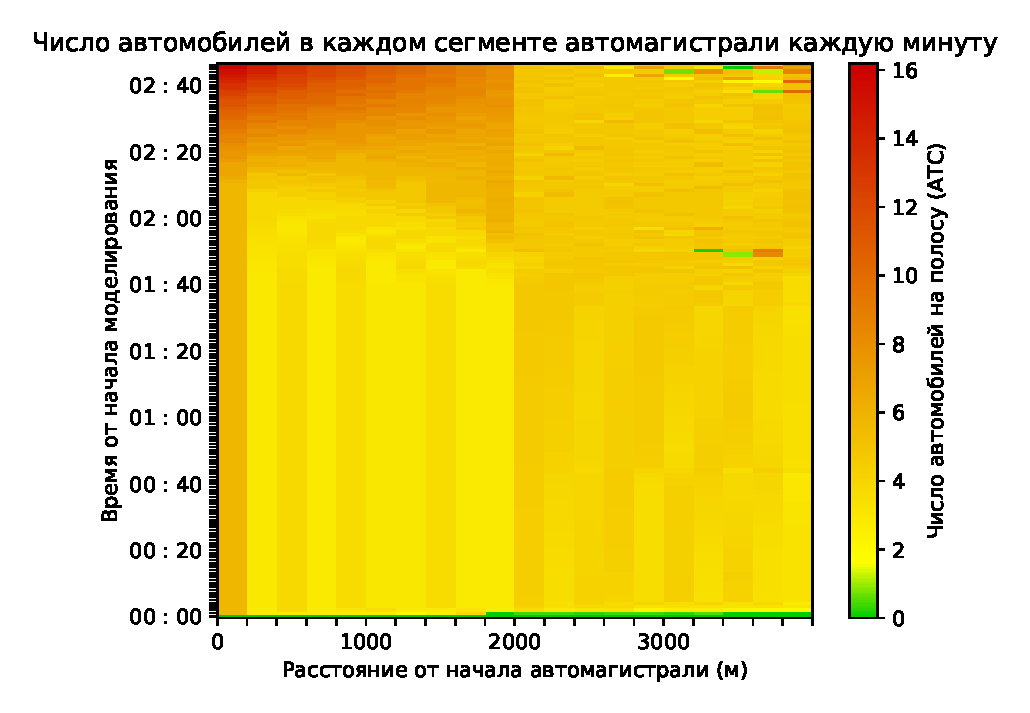
\includegraphics[width=1.0\linewidth]{jamming_crossroad_enter_5_2.eps}
       \caption{}
    \end{subfigure}

    \caption{а) Схема дороги. б) Тепловая карта автомобилей на пятиполосной дороге со въездом с постепенно нарастающем потоком с него.}
    \label{fig:jamming_crossroad_enter_5_1}
\end{figure}

\section{Данные дорожных датчиков}
\subsection{Прямая дорога}
\label{sec::experiment_1}
В данном эксперименте мы воспользовались построенной для данного участка автомагистрали фундаментальной диаграммой~\cite{collectiveArticle2}.
Полный временной интервал эксперимента~--- одна неделя, графики приведены за один день.
В приведенном эксперименте проводится проверка результатов модели в простейшем случае моделирования числа съехавших АТС по числу въехавших на участке автомагистрали без въездов и съездов.
Результаты видны на графике~\ref{fig:MCAR_simple_test}.
\begin{figure}[ht]
    \centerfloat{
        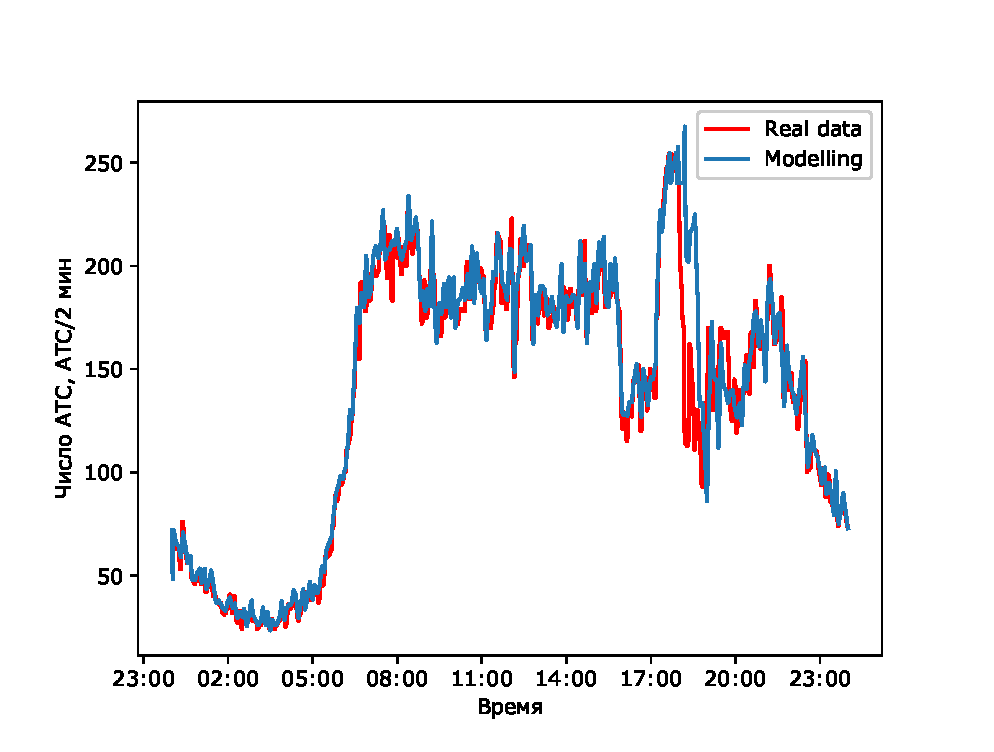
\includegraphics[width=1.0\linewidth]{MCAR_simple_test.eps}
    }
    \caption{График полученного с помощью модели числа съехавших АТС (красная линия) в сравнении с числом съехавших АТС зафиксированных дорожным датчиком (синяя линия) за один день. Среднеквадратичная ошибка $S = 18.4$.}
    \label{fig:MCAR_simple_test}
\end{figure}
Среднеквадратичная ошибка $S = 18.4$.

\subsection{Эксперимент с перекрытием полосы}
\label{sec::experiment_2}
Во втором эксперименте на основе реальных данных проводится моделирование ситуации, когда одна из полос на автомагистрали перекрывается.
Сам эксперимент проводится на том же участке автомагистрали и за тот же промежуток времени, что и первый в разделе~\ref{sec::experiment_1}.
В данном эксперименте у нас нет данных для расчета среднеквадратичной ошибки и он был поставлен для рассмотрения поведения модели в данной ситуации.
Результаты за тот же день, что и в первом эксперименте на данных дорожных датчиков можно увидеть на графике~\ref{fig:MCAR_minus_road_test}.
\begin{figure}[ht]
    \centerfloat{
        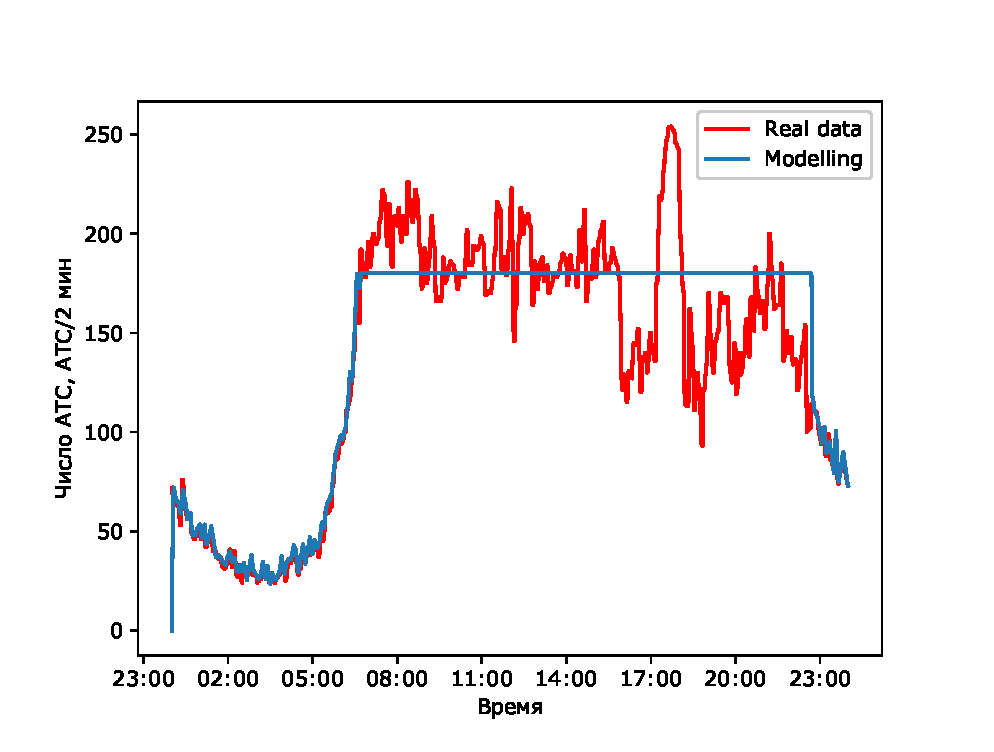
\includegraphics[width=1.0\linewidth]{MCAR_minus_line.eps}
    }
    \caption{График полученного с помощью модели числа съехавших АТС (красная линия) в сравнении с числом съехавших АТС зафиксированных дорожным датчиком (синяя линия) за один день.}
    \label{fig:MCAR_minus_road_test}
\end{figure}

Видно, что АТС не могут съехать из за того, что пропускная способность автомагистрали снизилась, что приводит к появлению горизонтальной линии на графике.
Однако, через некоторое время после того как поток должен был спасть, что видно на графике реальных данных за тот же временной промежуток, дорога освобождается и результат моделирования приходит в соответствие с реальными данными.

\section{Обсуждение результатов раздела}
Эксперименты из данной главы показывают работоспособность модели для моделирования всевозможных конфигураций автомагистрали при любом потоке АТС на ней.
Показано, что модель адекватно симулирует поведение АТС на автомагистрали как в ситуации достаточной ее пропускной способности, так и при ее превышении, а также моделирует различные варианты образования заторных ситуации как при распространении пробки из за проблем на магистрали на фиг.~\ref{fig:jammed_5-2_3block_road_sin_wave}, так и по причине недостаточной пропускной способности прилегающих съездов~\ref{fig:jamming_crossroad_exit_5_1}.

Также на реальных данных видно~\ref{fig:MCAR_simple_test}, что в модели нет потери автомобилей и она моделирует реальный участок автомагистрали в соответствии с зафиксированными дорожными датчиками данными.
Тут надо также понимать, что полученная небольшая ошибка связана как с несовершенством модели, так и с ошибками в видеофиксации дорожными датчиками.

Эксперимент изображенный на~\ref{fig:MCAR_minus_road_test} показывает состоятельность модели при перекрытии части автомагистрали~--- видно, что при уменьшении потока АТС пробка исчезает и результаты приходят в соответствие с реальными данными.

\FloatBarrier 